\documentclass{beamer}
\usetheme{Warsaw}

\usepackage{mathtools}
\usepackage{graphicx}

\title{Proof For Closed Eulerian Trails}
\author[Graham Swain]{Graham Swain}
\date{September 13, 2022 \\ Math 479}

\begin{document}
    
\frame{\titlepage}

\section{Definitions}

\begin{frame}[t]
	\only<1->{
		\begin{definition}
			A {\bf walk} is a sequence of vertices in which each consecutive pair of vertices are adjacent.
		\end{definition}
	}
	\only<2->{
		\begin{definition}
			A {\bf trail} is a walk where edges are not allowed to be repeated.
			\begin{itemize}
				\item<3-> It is called a {\bf closed trail} when it begins and ends at the same vertex.
			\end{itemize}
		\end{definition}
	}
	\only<4->{
		\begin{definition}
			If a trail uses all the edges in a graph it is called a {\bf Eulerian trail}.
			\begin{itemize}
				\item<5-> A {\bf closed Eulerian trail} is when an Eulerian trail begins and ends 
				on the same vertex. 
			\end{itemize} 
		\end{definition}
	}
\end{frame}

\begin{frame}[t]
	\only<1->{
		\begin{definition}
			A graph is {\bf connected} if, and only if, there is a walk between any two vertices $v$ and $w$.
		\end{definition}
	}

	\only<2>{
		\hspace{0.5in}
		\begin{definition}
			The {\bf degree} of a vertex, $v$, is the number of edges incident with $v$.
		\end{definition}
	}
\end{frame}

\section{Theorem and Proof}

\begin{frame}
	\begin{theorem}[Euler]
		A connected graph has a closed Eulerian trail if and only if all of its vertices have 
		even degree.
	\end{theorem}
\end{frame}


\begin{frame}[t]
	\begin{proof}\renewcommand{\qedsymbol}{}
		\begin{enumerate}
			\item[$\Rightarrow$]
			Assume a connected graph $G$ has a closed Eulerian trail, denoted as $C$. Prove that every
			vertex has an even degree.
		\end{enumerate}
		Take an arbitrary vertex $v$. As we traverse $C$, each time we enter $v$ we must be able
		to exit on a distinct edge. Thus every vertex must be adjacent to $2k$ edges, where $k$
		is the number of times a vertex is visited. Therefore every vertex has even degree.
	\end{proof}

	\begin{figure}
		\centering
		\only<2>{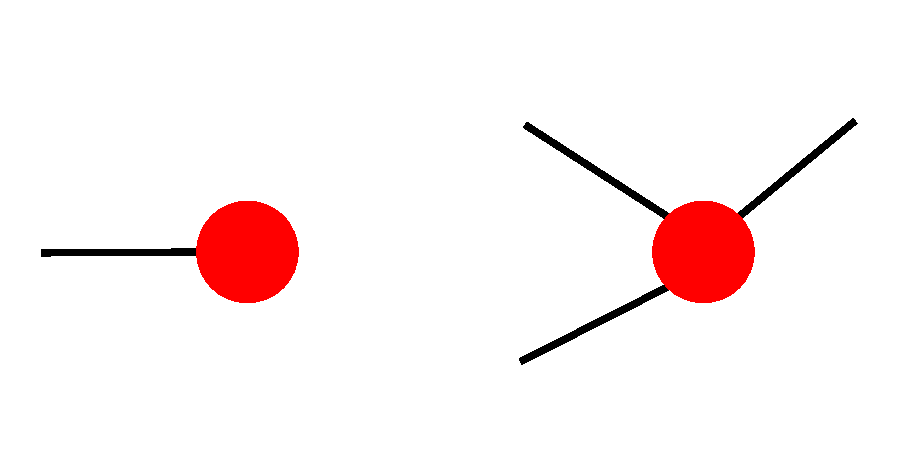
\includegraphics[scale=.4]{pictures/bad_examples.pdf}}
		\only<3>{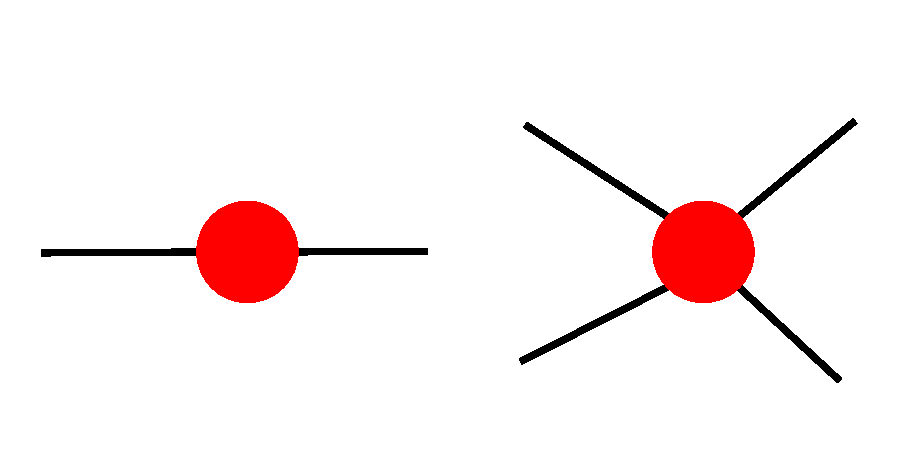
\includegraphics[scale=.4]{pictures/good_examples.pdf}}
	\end{figure}
\end{frame}

\begin{frame}[t]
	\begin{proof}[Proof (cont)]
		\only<1>{
		\begin{enumerate}
			\item[$\Leftarrow$]
			Assume $G$ is a connected graph with every vertex having even degree. Prove that it has
			a closed Eulerian trail.
		\end{enumerate}}

		\only<2-3>{Starting at an arbitrary vertex $v$, begin constructing a trail. Continue until we reach a vertex
		we cannot leave. If this vertex is not $v$, we entered on one edge and do not have a
		corresponding exit, meaning this vertex has an odd degree, which is a contradiction.
		So we know that it is $v$, meaning we have found a closed trail, which we will called
		$C_1$.}
		
		\only<4-5>{If $C_1$ contains all the edges of $G$, we have found an Eulerian trail and are 
		done, if not remove all the edges of $C_1$ from $G$, let's call the resulting graph $G'$. 
		$G'$ is not necessarily connected.}

		\only<6>{Select a vertex $w$ that is in both $C_1$ and $G$. Then begin tracing 
		a trail in $G'$ Starting at $w$ until we arrive back at $w$. Name the resulting closed 
		trail $C_2$.}
		
		\only<7>{Combine $C_1$ and $C_2$ to form another closed trail denoted as $C'$. If 
		$C'$ contains all the edges of $G$, we have found a closed Eulerian trail. If not, 
		remove all the edges of $C'$ from $G$ to get $G''$. Choose a vertex in both $C'$ and 
		$G''$ and repeat the steps above until we have used all the edges of $G$.}
		\alt<7>{\qedhere}{\phantom\qedhere}
	\end{proof}
	
	\begin{figure}
		\centering
		\only<1>{\includegraphics[scale=.25]{pictures/g.pdf}}
		\only<3-4>{\includegraphics[scale=.25]{pictures/c1.pdf}}
		\only<5>{\includegraphics[scale=.25]{pictures/g'.pdf}}
		\only<6>{\includegraphics[scale=.25]{pictures/c2.pdf}}
		\only<7>{\includegraphics[scale=.25]{pictures/c'.pdf}}
	\end{figure}
\end{frame}

\begin{frame}
	\begin{figure}
		\centering
		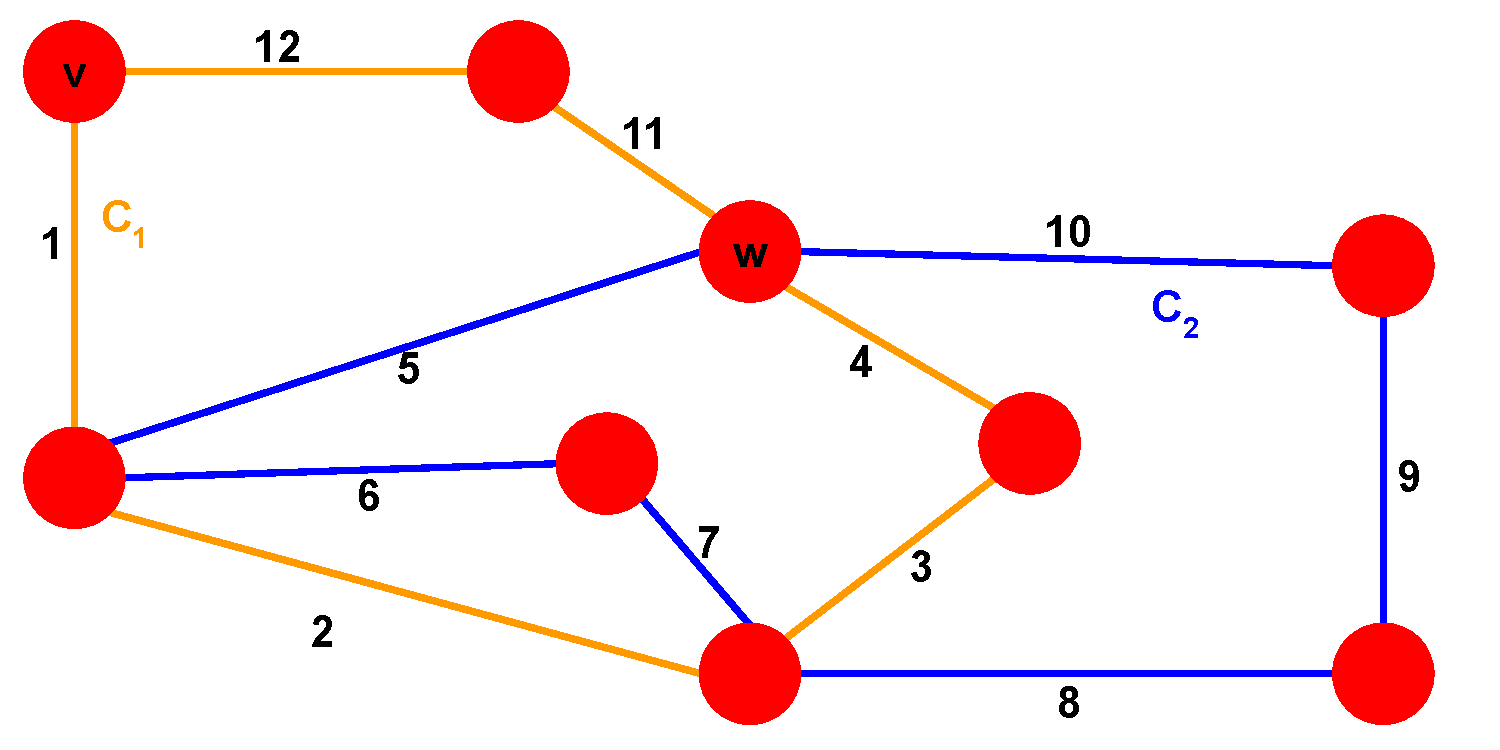
\includegraphics[scale=.40]{pictures/c'_traversal.pdf}
	\end{figure}
\end{frame}

\begin{frame}[t]
	\begin{proof}[Proof cont.]
		Combine $C_1$ and $C_2$ to form another closed trail denoted as $C'$. If 
		$C'$ contains all the edges of $G$, we have found a closed Eulerian trail. If not, 
		remove all the edges of $C'$ from $G$ to get $G''$. Choose a vertex in both $C'$ and 
		$G''$ and repeat the steps above until we have used all the edges of $G$.
	\end{proof}

	\begin{figure}
		\centering
		\includegraphics[scale=.25]{pictures/c'.pdf}
	\end{figure}
\end{frame}

\section{Conclusion}

\frame{
	\frametitle{References}
	\begin{enumerate}{\scriptsize
		\item[{[1]}] Belcastro, {\it Discrete Mathematics with Ducks}, CRC Press, 2012.
		\item[{[2]}] Epp, {\it Discrete Mathematics with Applications}, Brooks Cole, 1996.
		
		}\end{enumerate}

}

\end{document}